% Dieser Text ist urheberrechtlich gesch�tzt
% Er stellt einen Auszug eines von mir erstellten Referates dar
% und darf nicht gewerblich genutzt werden
% die private bzw. Studiums bezogen Nutzung ist frei
% Mai. 2007
% Autor: Sascha Frank 
% Universit�t Freiburg 
% www.informatik.uni-freiburg.de/~frank/
\documentclass{beamer}
\usepackage{pst-bar,pst-plot,pstricks-add}
\usepackage{graphics,graphicx}
\usepackage{pstricks,pst-node,pst-tree}

% \usepackage{graphicx}
\setbeamertemplate{navigation symbols}{}
% \usepackage{beamerthemeshadow}
\beamersetuncovermixins{\opaqueness<1>{25}}{\opaqueness<2->{15}}
\usetheme{CambridgeUS}
\usecolortheme{whale}

\begin{document}
\title{The max-min-hill-climbing algorithm}  
\author[M. Bauer]{Michael Bauer}
\institute[M.Sc. Comp. Science]{M.Sc. Comp. Science}
\date{\today}
% \begin{document}
% \title{Beamer Class ganz nett}  
% \author{Sascha Frank}
% \date{\today} 

\begin{frame}
\titlepage
\end{frame} 

% \begin{frame}
% \tableofcontents
% \end{frame} 

\section{Introduction} 
	\begin{frame}
		\begin{center}
			\begin{huge}
				Learning a graph and its structure
			\end{huge}
		\end{center}
	\end{frame}

		\subsection{Learning a graph and its structure}
		\begin{frame}
			\center
				$
					\psmatrix[colsep=1.2cm,rowsep=1cm,mnode=circle]
					&Difficulty&&Intelligence\\
					&&Grade&&SAT\\
					&&Letter
					\ncline{->}{1,2}{2,3}
					\ncline{->}{1,4}{2,3}
					\ncline{->}{1,4}{2,5}
					\ncline{->}{2,3}{3,3}
					\endpsmatrix
				$
		\end{frame}

\section{Graph theory} 
	\begin{frame}
		\begin{center}
			\begin{huge}
				Graph theory
			\end{huge}
		\end{center}
	\end{frame}
	\subsection{DAG (directed acyclic graph)}
		\begin{frame}
			Directed Acyclic Graph

			\center
				$
					\psmatrix[colsep=1.8cm,rowsep=1cm,mnode=circle]
					&1&&2\\
					&&3&&4\\
					&&5
					\ncline{->}{1,2}{2,3}
					\ncline{->}{1,4}{2,3}
					\ncline{->}{1,4}{2,5}
					\ncline{->}{2,3}{3,3}
					\endpsmatrix
				$
		\end{frame}

	\subsection{Bayesian Network}
		\begin{frame}
			Bayesian Network

			\center
				$
					\psmatrix[colsep=1.2cm,rowsep=1cm,mnode=circle]
					&parent&&parent\\
					&&child \& parent&&child\\
					&&child
					\ncline{->}{1,2}{2,3}
					\ncline{->}{1,4}{2,3}
					\ncline{->}{1,4}{2,5}
					\ncline{->}{2,3}{3,3}
					\endpsmatrix
				$
		\end{frame}

\section{Probability theory}
	\begin{frame}
		\begin{center}
			\begin{huge}
				Probability theory
			\end{huge}
		\end{center}
	\end{frame}
	\subsection{Independence and Conditional Probability}
		\begin{frame}
			\center
			\begin{Large}
				Reminder
			\end{Large}
			\begin{block}{Definition (Independence)}
				Let $A$, $B$ denote random variables. Then $A$ and $B$ are independent iff
					\begin{equation}
						P(A \cap B) = P(A)*P(B)
					\end{equation}
			\end{block}
			\begin{block}{Definition (Conditional Probability)}
				Let $A$, $B$ denote random variables and $P(B) > 0$. The probability of $A$ given $B$ is defined as:
					\begin{equation}
						P(A | B) = \frac{P(A \cap B)}{P(B)}
					\end{equation}
			\end{block}
		\end{frame}
	
	\begin{frame}
		\begin{center}
			\begin{huge}
				Combining these approaches
			\end{huge}
		\end{center}
	\end{frame}

	\subsection{Conditional Independence}
		\begin{frame}
			\center
			\begin{block}{Definition (Conditional Independence)}
				Two variables $X$ and $Y$ are \underline{conditionally independent given \textbf{Z}} w.r.t a probability distribution P, denoted as $Ind_{p}(X;Y|\textbf{Z})$, if $\forall x,y,\textbf{z}$, where $P(\textbf{Z} = \textbf{z}) > 0$,
					\begin{equation}
						P(X,Y|\textbf{Z}) = P(X|\textbf{Z})*P(Y|\textbf{Z})
					\end{equation}
				where $P(X,Y|\textbf{Z}) = P(X \cap Y|\textbf{Z})$.
			\end{block}
		\end{frame}

\section{Computational properties}
	\begin{frame}
		\begin{center}
			\begin{huge}
				Computational properties
			\end{huge}
		\end{center}
	\end{frame}
	\subsection{The MMHC}
		\begin{frame}
			\center
			\begin{block}{Remark to MMHC}
				\begin{itemize}
					\item  Greedy Algorithm \pause
					\item  Constrained-based \pause
					\item  A hybrid algorithm \pause
					\item  np-hard
				\end{itemize} 
			\end{block}
		\end{frame}

% \begin{frame}\frametitle{Aufz\"ahlung mit Pausen}
% \begin{itemize}
% \item  Einf\"uhrungskurs in \LaTeX \pause 
% \item  Kurs 2 \pause 
% \item  Seminararbeiten und Pr\"asentationen mit \LaTeX \pause 
% \item  Die Beamerclass
% \end{itemize} 
% \end{frame}

\subsection{Listen II}
\begin{frame}\frametitle{Numerierte Liste}
\begin{enumerate}
\item  Einf\"uhrungskurs in \LaTeX 
\item  Kurs 2
\item  Seminararbeiten und Pr\"asentationen mit \LaTeX 
\item  Die Beamerclass
\end{enumerate}
\end{frame}
\begin{frame}\frametitle{Numerierte Liste mit Pausen}
\begin{enumerate}
\item  Einf\"uhrungskurs in \LaTeX \pause 
\item  Kurs 2 \pause 
\item  Seminararbeiten und Pr\"asentationen mit \LaTeX \pause 
\item  Die Beamerclass
\end{enumerate}
\end{frame}

\section{Abschnitt Nr.3} 
\subsection{Tabellen}
\begin{frame}\frametitle{Tabellen}
\begin{tabular}{|c|c|c|}
\hline
\textbf{Zeitpunkt} & \textbf{Kursleiter} & \textbf{Titel} \\
\hline
WS 04/05 & Sascha Frank &  Erste Schritte mit \LaTeX  \\
\hline
SS 05 & Sascha Frank & \LaTeX \ Kursreihe \\
\hline
\end{tabular}
\end{frame}


\begin{frame}\frametitle{Tabellen mit Pause}
\begin{tabular}{c c c}
A & B & C \\ 
\pause 
1 & 2 & 3 \\  
\pause 
A & B & C \\ 
\end{tabular} 
\end{frame}


\section{Abschnitt Nr. 4}
\subsection{Bl\"ocke}
\begin{frame}\frametitle{Bl\"ocke}

\begin{block}{Blocktitel}
Blocktext 
\end{block}

\begin{exampleblock}{Blocktitel}
Blocktext 
\end{exampleblock}


\begin{alertblock}{Blocktitel}
Blocktext 
\end{alertblock}
\end{frame}

% \section{Abschnitt Nr. 5}
% \subsection{Geteilter Bildschirm}

% \begin{frame}\frametitle{Zerteilen des Bildschirmes}
% \begin{columns}
% \begin{column}{5cm}
% \begin{itemize}
% \item Beamer 
% \item Beamer Class 
% \item Beamer Class Latex 
% \end{itemize}
% \end{column}
% \begin{column}{5cm}
% \begin{tabular}{|c|c|}
% \hline
% \textbf{Kursleiter} & \textbf{Titel} \\
% \hline
% Sascha Frank &  \LaTeX \ Kurs 1 \\
% \hline
% Sascha Frank & \LaTeX \ Kursreihe \\
% \hline
% \end{tabular}
% \end{column}
% \end{columns}
% \end{frame}

% \subsection{Bilder} 
% \begin{frame}\frametitle{Bilder in Beamer}
% \begin{figure}
% 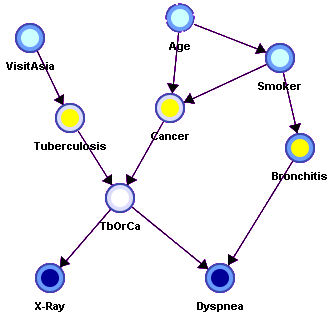
\includegraphics[scale=0.5]{bn.png} 
% \caption{Die Abbildung zeigt ein Beispielbild}
% \end{figure}
% \end{frame}


% \subsection{Bilder und Listen kombiniert} 

% \begin{frame}
% \frametitle{Bilder und Itemization in Beamer}
% \begin{columns}
% \begin{column}{5cm}
% \begin{itemize}
% \item<1-> Stichwort 1
% \item<3-> Stichwort 2
% \item<5-> Stichwort 3
% \end{itemize}
% \vspace{3cm} 
% \end{column}
% \begin{column}{5cm}
% \begin{overprint}
% \includegraphics<2>{PIC1}
% \includegraphics<4>{PIC2}
% \includegraphics<6>{PIC3}
% \end{overprint}
% \end{column}
% \end{columns}
% \end{frame}

% \subsection{Bilder die mehr Platz brauchen} 
% \begin{frame}[plain]
% \frametitle{plain, oder wie man mehr Platz hat}
% \begin{figure}
% \includegraphics[scale=0.5]{PIC1} 
% \caption{Die Abbildung zeigt ein Beispielbild}
% \end{figure}
% \end{frame}

\end{document}